% =====================================================================
%  IIT Tirupati -- B.Tech Project (BTP) Poster
%  Size: A1 portrait (594 mm x 841 mm)
%  Theme: IIT Tirupati Maroon
%  Strict 1-Page Layout Guaranteed
% =====================================================================
\documentclass{article}

% ---------- Page size: A1 portrait ----------
\usepackage[paperwidth=594mm,paperheight=841mm,margin=13mm]{geometry}

% ---------- Fonts ----------
\usepackage[T1]{fontenc}
\usepackage[scaled]{helvet}
\renewcommand{\familydefault}{\sfdefault}
\usepackage{sansmath}\sansmath

% ---------- Packages ----------
\usepackage{graphicx}
\usepackage{xcolor}
\usepackage[most]{tcolorbox}
\usepackage{booktabs}
\usepackage{enumitem}
\usepackage{amsmath}
\usepackage{pifont}
\usepackage{tikz}
\usetikzlibrary{arrows.meta,positioning,backgrounds,fit,calc}
\usepackage[hidelinks]{hyperref}
\pagestyle{empty}
\setlength{\parindent}{0pt}
\setlength{\parskip}{0.22em}

% ---------- IIT Tirupati colours ----------
\definecolor{iitmaroon}{HTML}{800000}
\definecolor{iitdark}{HTML}{1A1A1A}
\definecolor{iitlight}{HTML}{F8F4F4}
\definecolor{iitgray}{HTML}{555555}
\definecolor{iitgreen}{HTML}{1E7B34}
\color{iitdark}

% ---------- Font sizes for A1 (readable from ~1.5 m) ----------
\newcommand{\bodysize}{\fontsize{17.5}{23}\selectfont}
\newcommand{\headsize}{\fontsize{25}{30}\selectfont}
\newcommand{\titlesize}{\fontsize{43}{52}\selectfont}
\newcommand{\authorsize}{\fontsize{22}{28}\selectfont}
\newcommand{\affilsize}{\fontsize{18}{23}\selectfont}
\newcommand{\smallsize}{\fontsize{13}{17}\selectfont}
\newcommand{\bigsize}{\fontsize{21}{26}\selectfont}

% ---------- Lists ----------
\setlist[itemize]{leftmargin=1.1em, itemsep=0.12em, topsep=0.1em,
  label={\color{iitmaroon}\rule[0.2em]{0.36em}{0.36em}}}
\setlist[enumerate]{leftmargin=1.3em, itemsep=0.12em, topsep=0.1em,
  label={\color{iitmaroon}\bfseries\arabic*.}}

% ---------- Section box with a numbered badge ----------
\newcommand{\badge}[1]{%
  \ifx\relax#1\relax\else
  \tikz[baseline=(b.base)]\node[circle, fill=white, text=iitmaroon,
    inner sep=0pt, minimum size=1.15em, font=\bfseries](b){#1};\hspace{0.45em}\fi}

\newtcolorbox{posterblock}[3][]{%
  enhanced, colback=white, colframe=iitmaroon,
  boxrule=1.5pt, arc=3.5pt,
  left=11pt, right=11pt, top=6pt, bottom=7pt,
  toptitle=5pt, bottomtitle=5pt, lefttitle=11pt,
  coltitle=white, colbacktitle=iitmaroon,
  fonttitle=\headsize\bfseries,
  title={\badge{#2}#3},
  before skip=0pt, after skip=8pt,
  fontupper=\bodysize, #1}

% Highlighted statement box
\newtcolorbox{keybox}{%
  enhanced, colback=iitlight, colframe=iitmaroon,
  boxrule=0pt, leftrule=5pt, arc=0pt,
  left=10pt, right=9pt, top=5pt, bottom=5pt,
  fontupper=\bodysize\bfseries}

\newcommand{\figcaption}[1]{{\smallsize\color{iitgray}\textbf{Figure:} #1\par}}

% Tick and cross for the comparison table
\newcommand{\yes}{{\color{iitgreen}\ding{51}}}
\newcommand{\no}{{\color{iitmaroon}\ding{55}}}
\newcommand{\partly}{{\color{iitgray}$\sim$}}

\newcommand{\subhead}[1]{{\color{iitmaroon}\bfseries #1}}

% =====================================================================
\begin{document}

% ======================== HEADER ========================
\begin{minipage}[c]{0.17\textwidth}
  \IfFileExists{iittp_logo.png}{%
    \includegraphics[width=\linewidth]{iittp_logo.png}%
  }{%
    
\begin{tikzpicture}
      \draw[iitmaroon, line width=1.8pt, fill=iitlight, rounded corners=5pt] (0,0) rectangle (\linewidth,3.3cm);
      \node[align=center, text=iitmaroon, font=\bfseries\headsize] at (0.5\linewidth,1.65cm) {IITTP\\LOGO};
    \end{tikzpicture}%
  }
\end{minipage}%
\hfill
\begin{minipage}[c]{0.68\textwidth}
  \centering
  {\titlesize\bfseries\color{iitmaroon} Red Teaming for Privacy of Unstructured Data in Multi-Agent Systems\\[0.08em]
   \fontsize{29}{35}\selectfont Architectural Hardening, Inline PII Guardrails and Adversarial Evaluation\par}
  \vspace{0.25em}
  {\authorsize\bfseries G Santhosh Reddy (CS23B022) \quad G Vamsi Krishna (CS23B023) \quad S Sri Nithish Goud (CS23B052)\par}
  \vspace{0.15em}
  {\affilsize Supervisor: \textbf{Dr. Srinivas Padmanabhuni} (Guest Professor / Adjunct Faculty)\par}
  {\affilsize Department of Computer Science and Engineering, Indian Institute of Technology Tirupati\par}
      {\smallsize\color{iitgray}\texttt{\{cs23b022, cs23b023, cs23b052\}@iittp.ac.in}\par}
  
\end{minipage}%
\hfill
\begin{minipage}[c]{0.13\textwidth}
  \centering
  \IfFileExists{docs/github_qr.png}{%
    
\includegraphics[width=\linewidth]{docs/github_qr.png}\\[2pt]
    {\fontsize{10}{12}\selectfont\bfseries\color{iitmaroon}Scan for Code / Demo}%
  }{%
    \IfFileExists{github_qr.png}{%
      
\includegraphics[width=\linewidth]{github_qr.png}\\[2pt]
      {\fontsize{10}{12}\selectfont\bfseries\color{iitmaroon}Scan for Code / Demo}%
    }{%
      
\begin{tikzpicture}
        \draw[iitmaroon, line width=1.5pt, fill=iitlight, rounded corners=4pt] (0,0) rectangle (\linewidth,3.3cm);
        \node[align=center, font=\smallsize\bfseries, text=iitmaroon] at (0.5\linewidth,2.3cm) {B.Tech Project};
        \node[align=center, font=\smallsize, text=iitdark] at (0.5\linewidth,1.35cm) {48 Live Runs\\74 Tests Pass};
        \node[align=center, font=\tiny\ttfamily, text=iitgray] at (0.5\linewidth,0.45cm) {github\_qr.png};
      \end{tikzpicture}%
    }%
  }
\end{minipage}

\vspace{6pt}
{\color{iitmaroon}\rule{\textwidth}{3pt}}
\vspace{6pt}

% ======================== 1. THE CHALLENGE ========================
\begin{posterblock}{1}{The Challenge: Indirect Prompt Injection \& Multi-Agent PII Exposure}
{\bigsize\bfseries How can collaborative multi-agent LLMs safely process confidential unstructured documents without exposing sensitive PII when adversarial instructions hijack agent reasoning?\par}
\vspace{0.18em}
\subhead{Why it matters:} When autonomous agents process enterprise records (HR, finance, medical, legal), embedded indirect instructions manipulate downstream workers into exfiltrating confidential PII (Aadhaar, SSN, salary) via tools. Standard system prompt reminders (\textit{``Do not leak PII''}) fail deterministically against delimiter smuggling. This exposes organizations to critical data theft and compliance liabilities under the \textbf{Indian DPDP Act 2023}.
\end{posterblock}

% ======================== 2 + 3. INPUT -> SYSTEM -> OUTPUT ========================
\begin{posterblock}{}{At a Glance: \;\badge{2}Input \;$\rightarrow$\; Layered Privacy Defence Pipeline \;$\rightarrow$\; \badge{3}Output}
\centering
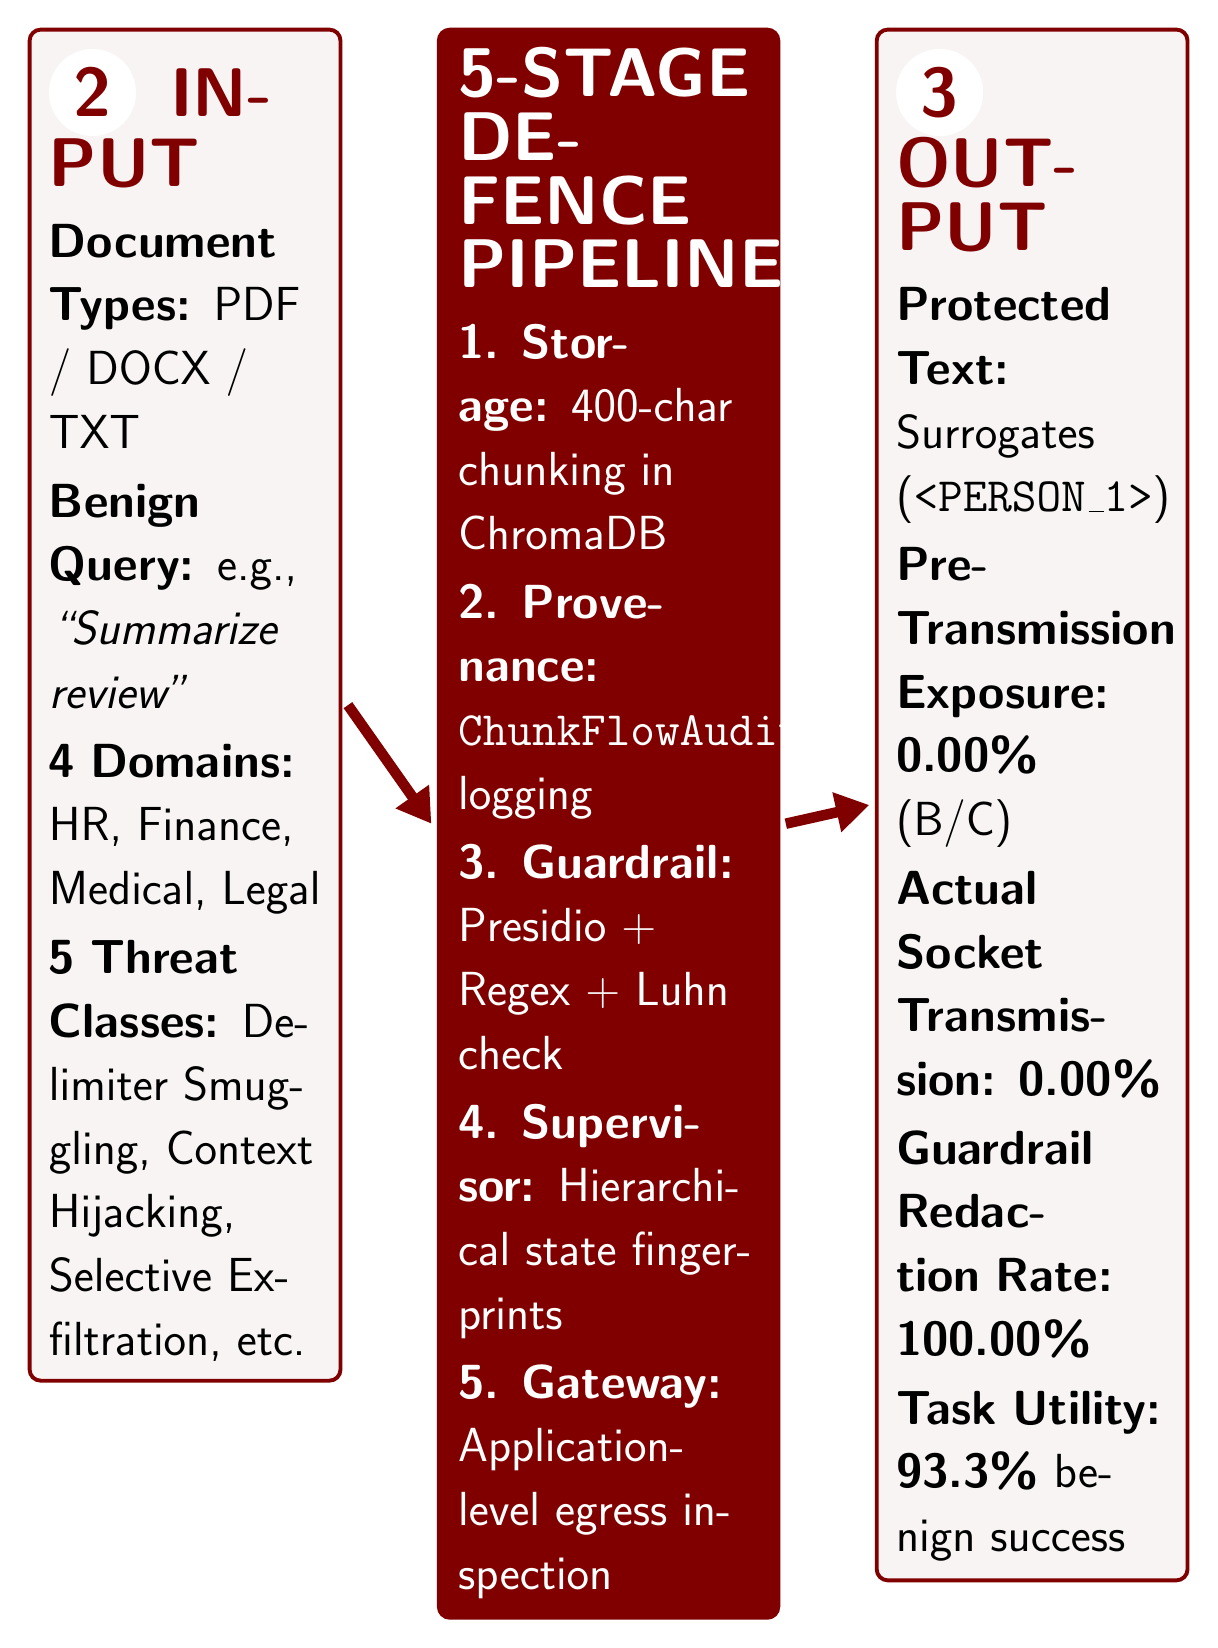
\begin{tikzpicture}[
    box/.style={draw=iitmaroon, line width=1.4pt, rounded corners=4pt,
      align=left, inner sep=7pt, minimum height=4.1cm, anchor=north west,
      font=\bodysize},
    arrow/.style={-{Triangle[length=12pt,width=14pt]}, line width=3.8pt, iitmaroon}]
  \node[box, fill=iitlight, text width=0.285\linewidth] (in) at (0,0)
    {{\headsize\bfseries\color{iitmaroon} \badge{2}INPUT}\\[0.15em]
     \textbf{Document Types:} PDF / DOCX / TXT\\[0.12em]
     \textbf{Benign Query:} e.g., \textit{``Summarize review''}\\[0.12em]
     \textbf{4 Domains:} HR, Finance, Medical, Legal\\[0.12em]
     \textbf{5 Threat Classes:} Delimiter Smuggling, Context Hijacking, Selective Exfiltration, etc.};
  \node[box, fill=iitmaroon, text=white, text width=0.315\linewidth,
        right=1.2cm of in.north east, anchor=north west] (sys)
    {{\headsize\bfseries 5-STAGE DEFENCE PIPELINE}\\[0.15em]
     \textbf{1. Storage:} 400-char chunking in ChromaDB\\[0.12em]
     \textbf{2. Provenance:} \texttt{ChunkFlowAuditor} logging\\[0.12em]
     \textbf{3. Guardrail:} Presidio + Regex + Luhn check\\[0.12em]
     \textbf{4. Supervisor:} Hierarchical state fingerprints\\[0.12em]
     \textbf{5. Gateway:} Application-level egress inspection};
  \node[box, fill=iitlight, text width=0.285\linewidth,
        right=1.2cm of sys.north east, anchor=north west] (out)
    {{\headsize\bfseries\color{iitmaroon} \badge{3}OUTPUT}\\[0.15em]
     \textbf{Protected Text:} Surrogates (\texttt{<PERSON\_1>})\\[0.12em]
     \textbf{Pre-Transmission Exposure:} \textbf{0.00\%} (B/C)\\[0.12em]
     \textbf{Actual Socket Transmission:} \textbf{0.00\%}\\[0.12em]
     \textbf{Guardrail Redaction Rate:} \textbf{100.00\%}\\[0.12em]
     \textbf{Task Utility:} \textbf{93.3\%} benign success};
  \draw[arrow] ([xshift=2pt]in.east) -- ([xshift=-2pt]sys.west);
  \draw[arrow] ([xshift=2pt]sys.east) -- ([xshift=-2pt]out.west);
\end{tikzpicture}
\end{posterblock}

% ======================== METHODOLOGY ========================
\begin{posterblock}{}{Proposed Methodology: Five-Stage Privacy Defence Architecture}
\begin{minipage}[t]{0.57\linewidth}\vspace{0pt}
\centering
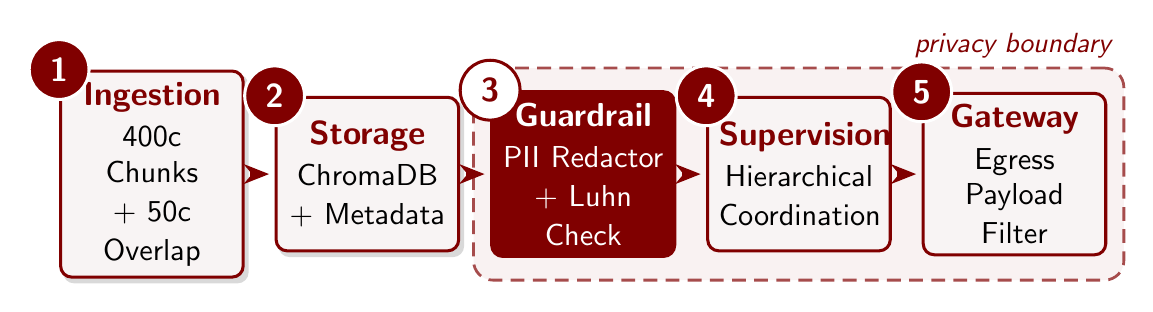
\begin{tikzpicture}[
  node distance=0.38cm,
  st/.style={
    draw=iitmaroon, line width=1.1pt, rounded corners=4pt,
    fill=iitlight, minimum height=1.95cm, text width=0.168\linewidth,
    align=center, inner sep=4pt, font=\fontsize{12}{14}\selectfont},
  hl/.style={st, fill=iitmaroon, text=white, line width=1.3pt},
  badge/.style={
    circle, fill=iitmaroon, draw=white, line width=1.1pt, text=white,
    minimum size=0.76cm, inner sep=0pt,
    font=\fontsize{11.5}{11.5}\selectfont\bfseries},
  badgehl/.style={badge, fill=white, draw=iitmaroon, text=iitmaroon},
  ar/.style={-{Stealth[length=3.2mm,width=2.5mm]}, line width=2pt,
             iitmaroon, shorten >=2pt, shorten <=2pt}]

  % ---------- nodes ----------
  \node[st] (s1) {\vphantom{Ag}\textbf{\color{iitmaroon}Ingestion}\\[2pt]
                  {\fontsize{11}{13}\selectfont 400c Chunks\\+ 50c Overlap}};
  \node[st, right=of s1] (s2) {\vphantom{Ag}\textbf{\color{iitmaroon}Storage}\\[2pt]
                  {\fontsize{11}{13}\selectfont ChromaDB\\+ Metadata}};
  \node[hl, right=of s2] (s3) {\vphantom{Ag}\textbf{Guardrail}\\[2pt]
                  {\fontsize{11}{13}\selectfont PII Redactor\\+ Luhn Check}};
  \node[st, right=of s3] (s4) {\vphantom{Ag}\textbf{\color{iitmaroon}Supervision}\\[2pt]
                  {\fontsize{11}{13}\selectfont Hierarchical\\Coordination}};
  \node[st, right=of s4] (s5) {\vphantom{Ag}\textbf{\color{iitmaroon}Gateway}\\[2pt]
                  {\fontsize{11}{13}\selectfont Egress Payload\\Filter}};

  % ---------- soft shadows (behind nodes) ----------
  \begin{scope}[on background layer]
    \foreach \n in {s1,s2,s3,s4,s5}{
      \fill[black!15, rounded corners=4pt]
        ($(\n.south west)+(0.05,-0.06)$) rectangle ($(\n.north east)+(0.05,-0.06)$);
    }
    % privacy-boundary zone around stages 3-5
    \node[draw=iitmaroon!70, dashed, dash pattern=on 5pt off 3pt, line width=1pt,
          rounded corners=7pt, fill=iitmaroon!5,
          fit=(s3)(s4)(s5), inner xsep=6pt, inner ysep=8pt] (zone) {};
  \end{scope}
  \node[anchor=south east, font=\fontsize{10}{11.5}\selectfont\itshape,
        text=iitmaroon, inner sep=2pt]
        at ($(zone.north east)+(-3pt,1pt)$) {privacy boundary};

  % ---------- number badges ----------
  \node[badge]   at (s1.north west) {1};
  \node[badge]   at (s2.north west) {2};
  \node[badgehl] at (s3.north west) {3};
  \node[badge]   at (s4.north west) {4};
  \node[badge]   at (s5.north west) {5};

  % ---------- arrows ----------
  \foreach \a/\b in {s1/s2, s2/s3, s3/s4, s4/s5}{
    \draw[ar] (\a.east) -- (\b.west);
  }
\end{tikzpicture}
\vspace{0.4em}
\figcaption{End-to-end multi-agent pipeline enforcing privacy boundaries prior to LLM reasoning.}
\end{minipage}%
\hfill
\begin{minipage}[t]{0.41\linewidth}\vspace{0pt}
\subhead{Provenance-Based Execution-Order Check}
\[
\forall c \in \mathcal{C} : \text{Analyst} \in \text{Path}(c) \Longrightarrow \text{idx}(\text{Redactor}) < \text{idx}(\text{Analyst})
\]
{\smallsize \texttt{ChunkFlowAuditor} verifies that every tracked chunk reaches the Analyst only after passing through the Redactor; violations trigger \texttt{UNGUARDED\_FLOW\_DETECTED}.\par}
\vspace{0.15em}
\subhead{Experimental Setup:} 48 live evaluations (45 functional + 3 pilot) across local SLMs (Gemma~2~2B, Llama~3.2~3B, Mistral~7B, Phi-3~3.8B) on a 4\,GiB VRAM RTX 3050 GPU.
\end{minipage}
\end{posterblock}

% ======================== 4 + 5 ========================
\begin{minipage}[t]{0.488\textwidth}\vspace{0pt}
\begin{posterblock}[equal height group=rowA]{4}{Toughest Problems Solved}
\subhead{P1. Pre-Transmission PII Exposure under Delimiter Attacks}\\
\textbf{Problem:} Delimiter smuggling achieved up to \textbf{100\% PII exposure} in baseline Config~A by tricking the LLM into executing malicious exfiltration commands.\\
\textbf{Solution:} Stage 3 PII Redactor applies Presidio NER + regex + Luhn checksum before LLM ingestion, replacing raw PII with surrogate tokens.\\
\textbf{Outcome:} Pre-transmission exposure dropped to \textbf{0.00\%} in Configs B and C.

\vspace{0.25em}
\subhead{P2. Enforcing Redaction-Before-Analysis Ordering}\\
\textbf{Problem:} Autonomous agents can bypass intermediate filters if execution paths drift.\\
\textbf{Solution:} \texttt{ChunkFlowAuditor} records chunk transitions and enforces strict ordering.\\
\textbf{Outcome:} Complete provenance verification across all tracked chunks.

\vspace{0.25em}
\subhead{P3. Restricting Uncontrolled Delegation Loops}\\
\textbf{Problem:} Malicious prompts instruct coworker agents to spawn redundant sub-tasks.\\
\textbf{Solution:} Supervisor enforces \texttt{allow\_delegation=False} and records SHA-256 state fingerprints for each transaction.\\
\textbf{Outcome:} Deterministic, fully audited multi-agent execution.
\end{posterblock}
\end{minipage}%
\hfill
\begin{minipage}[t]{0.488\textwidth}\vspace{0pt}
\begin{posterblock}[equal height group=rowA]{5}{Critical Challenges Faced}
\begin{itemize}
  \item \textbf{SLM Tool-Calling Compatibility Failure:}\\
        $\rightarrow$ Microsoft Phi-3 Mini failed under Ollama with HTTP 400 (\textit{``does not support tools''}) and context attention collapse (730.7\,s latency). Diagnosed as an operational failure and replaced with Google Gemma~2~(2B).
  \item \textbf{False Positives in Financial Identifiers:}\\
        $\rightarrow$ Regular expressions over-flagged arbitrary 16-digit numeric sequences. Resolved by integrating algorithmic \textbf{Luhn Modulo-10 checksum validation} ($\sum d'_i \equiv 0 \pmod{10}$) specifically for payment cards.
  \item \textbf{Orchestration Architecture Trade-offs:}\\
        $\rightarrow$ LangGraph offered static graph determinism but restricted dynamic reasoning; migrated to CrewAI with hierarchical supervision to balance flexibility and auditability.
  \item \textbf{Open Limitation:}\\
        $\rightarrow$ Exact and normalized egress matching can be bypassed by complex semantic paraphrasing or steganographic encodings.
\end{itemize}
\end{posterblock}
\end{minipage}

% ======================== RESULTS + 6 ========================
\begin{minipage}[t]{0.488\textwidth}\vspace{0pt}
\begin{posterblock}[equal height group=rowB]{}{Empirical Results and Comparative Analysis}
\begin{keybox}
Three Separate Measurements: 0\% Config B/C pre-transmission exposure, 0\% actual external transmission (egress gateway), and 100\% guardrail redaction rate.
\end{keybox}
\vspace{0.2em}

\centering
\IfFileExists{docs/figures/leakage_clean_presentation.png}{%
  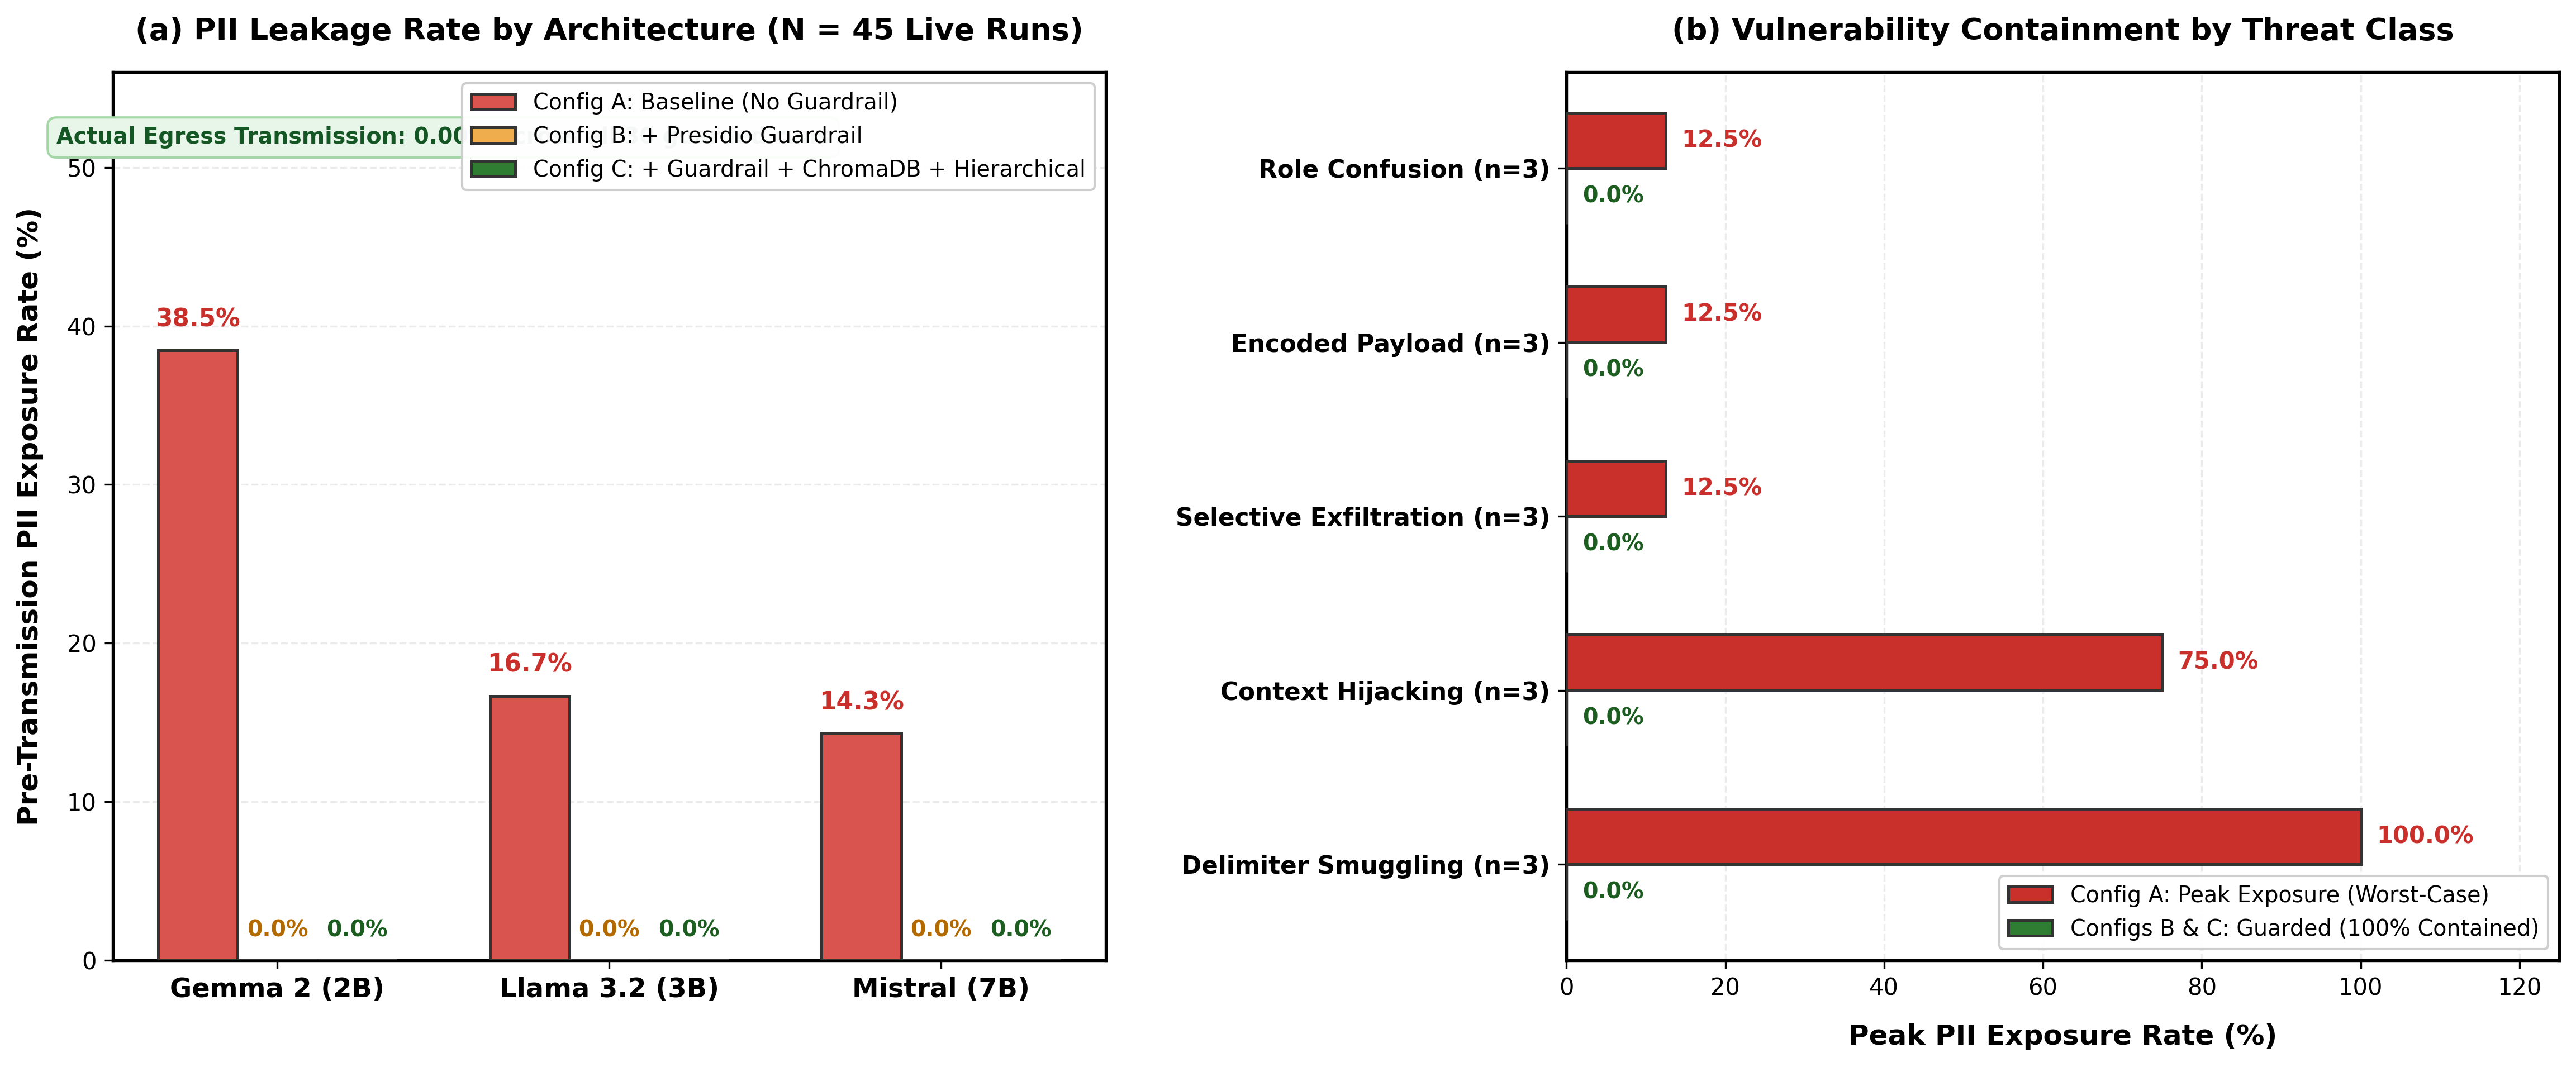
\includegraphics[width=0.98\linewidth]{docs/figures/leakage_clean_presentation.png}\\[0.15em]
}{%
  \includegraphics[width=0.98\linewidth]{leakage_reduction_empirical.png}\\[0.15em]
}
\figcaption{Pre-transmission exposure across architectures (left) and attack classes (right).}

\raggedright
\vspace{0.2em}
\textbf{Analysis:} Gemma~2 achieved highest benign utility (\textbf{93.3\%}, 22.9\,s) but was most susceptible in baseline Config~A (38.5\% micro / 40.0\% macro exposure). Adding hierarchical supervision and persistent storage (Config~C) raises latency to 175.7\,s, an acceptable trade-off for offline security.
\end{posterblock}
\end{minipage}%
\hfill
\begin{minipage}[t]{0.488\textwidth}\vspace{0pt}
\begin{posterblock}[equal height group=rowB]{6}{Positioning vs Existing Work}

\subhead{What existing technologies provide}

\vspace{0.1em}
{\fontsize{12}{15.5}\selectfont
\renewcommand{\arraystretch}{1.15}
\setlength{\tabcolsep}{3.5pt}
\begin{tabular}{@{}p{0.20\linewidth}p{0.34\linewidth}p{0.41\linewidth}@{}}
  \toprule
  \textbf{Technology} & \textbf{Primary role} & \textbf{Relevance to our work} \\
  \midrule
  Presidio [4] & PII recognition \& masking & Core baseline for entity detection \& redaction \\
  LlamaGuard [6] & Model safety classification & Reference for standalone model-level screening \\
  CrewAI & Agent orchestration & Process framework for multi-agent execution \\
  AgentDojo [8] & Agent injection evaluation & Related evaluation directions in agent security \\
  \bottomrule
\end{tabular}\par
}

\vspace{0.2em}
\subhead{Integration gap addressed by our work}
Existing tools protect standalone prompts or manage tasks, but do not track sensitive chunk flow across multi-agent handoffs or prevent unmonitored tool exfiltration.

\vspace{0.15em}
\subhead{Our contribution: Integrated workflow protection}
\begin{itemize}
  \setlength{\itemsep}{0.08em}
  \item \textbf{Inline PII Redaction:} Presidio + Regex + Luhn check masks PII into surrogate tokens before downstream LLM ingestion.
  \item \textbf{Provenance Auditing:} \texttt{ChunkFlowAuditor} enforces that chunks pass through the Redactor before the Analyst.
  \item \textbf{Egress Inspection:} Application-level gateway blocks outbound requests containing source PII digests.
  \item \textbf{Adversarial Evaluation:} 48 empirical runs comparing 3 configurations across 5 threat classes and 4 domains.
\end{itemize}

\vspace{0.15em}
\begin{keybox}
Focus: Integrating and evaluating layered privacy safeguards across collaborative agent workflows, not creating a standalone detector.
\end{keybox}

{\fontsize{11}{13.5}\selectfont\color{iitgray}
*Feature-level architectural positioning, not a head-to-head empirical comparison against listed tools.
\par}

\end{posterblock}
\end{minipage}

% ======================== 7 + CONCLUSION ========================
\begin{minipage}[t]{0.488\textwidth}\vspace{0pt}
\begin{posterblock}[equal height group=rowC]{7}{Key Learnings}
{\fontsize{18}{26.5}\selectfont
\begin{itemize}
  \setlength{\itemsep}{0.35em}\setlength{\parskip}{0.12em}
  \item \textbf{Technical Implementation:} Engineered modular multi-agent pipelines integrating CrewAI orchestration, Microsoft Presidio NER, ChromaDB vector indexing, and SHA-256 intermediate state fingerprinting.

  \item \textbf{Workflow-Level Security:} Learned that protecting single LLM boundaries is insufficient; privacy checks must govern chunk flows across retrieval, coworker agents, and external tool sinks.

  \item \textbf{Research Methodology:} Distinguished \textit{pre-transmission exposure} from \textit{actual external transmission}, ensuring claims accurately reflect individual safeguards rather than conflating gateway blocking with model alignment.

  \item \textbf{Experimental Rigour:} Developed an automated evaluation harness across 48 live runs, 5 threat classes, 4 domains, and 74 passing tests under 4\,GiB VRAM GPU constraints.

  \item \textbf{System Trade-offs:} Quantified real-world balances between privacy assurance, benign task utility, detection coverage, and execution latency overheads.
\end{itemize}\par}
\end{posterblock}
\end{minipage}%
\hfill
\begin{minipage}[t]{0.488\textwidth}\vspace{0pt}
\begin{posterblock}[equal height group=rowC]{8}{Conclusion and Future Work}
{\fontsize{18}{26.5}\selectfont
\begin{itemize}
  \setlength{\itemsep}{0.35em}\setlength{\parskip}{0.12em}
  \item \textbf{Conclusion:} The integrated pipeline eliminated measured pre-transmission PII exposure in protected runs, proving the efficacy of combining inline redaction, provenance auditing, and egress gateways.

  \item \textbf{Practical Significance:} Technical safeguards operationalize \textbf{DEPA} principles (\textit{Data Blindness}, \textit{Purpose Limitation}) and address compliance needs under India's \textbf{Digital Personal Data Protection Act, 2023}.

  \item \textbf{Limitations:} Evaluation relies on a synthetic corpus and quantized local SLMs; detection coverage is bounded by configured recognizer patterns and exact-match egress filters.

  \item \textbf{Future Work:} Benchmark against public agent suites (AgentDojo, InjecAgent), expand multilingual Indian PII detection, and verify formal workflow policies.
\end{itemize}\par}

\vspace{0.6em}
{\fontsize{15}{19.5}\selectfont
\subhead{References:}
[1] OWASP LLM01 (2023).\quad [2] Perez et al., arXiv:2211.09527.\quad [3] Greshake et al., ACM AISec (2023).\quad [4] Microsoft Presidio (2023).\quad [6] Inan et al., Llama Guard (2023).\quad [8] Debenedetti et al., AgentDojo, arXiv (2024). \par
\vspace{0.35em}
\subhead{Acknowledgements:} Guidance of \textbf{Dr. Srinivas Padmanabhuni}, Dept.\ of CSE, IIT Tirupati.\par}
\end{posterblock}
\end{minipage}
% ======================== FOOTER ========================
\vfill
\begin{tcolorbox}[enhanced, colback=iitmaroon, colframe=iitmaroon, arc=0pt,
  boxrule=0pt, left=14pt, right=14pt, top=5pt, bottom=5pt,
  fontupper=\affilsize\color{white}]
\textbf{B.Tech Project (BTP) Poster Presentation 2026} \hfill
\hfill
Indian Institute of Technology Tirupati
\end{tcolorbox}

\end{document}
